\documentclass{article}

\usepackage{graphicx}
\usepackage{float}
\usepackage{array}
\usepackage{amssymb}
\usepackage{amsmath}


\begin{document}

  \begin{titlepage}
    \centering
    \vspace*{2cm}
    
    \Huge
    \textbf{Simulador de Polarización en Redes}
    
    \vspace{1.5cm}
    
    \Large
    Jhorman Gomez{\textsuperscript{1}}, Ivan Ausecha{\textsuperscript{2}}, James Calero{\textsuperscript{3}}, Daniel Rojas{\textsubscript{4}}
    
    \vspace{0.5cm}
    
    \large
    2326867{\textsuperscript{1}}, -{\textsuperscript{2}}, -{\textsuperscript{3}}, 2040170{\textsuperscript{4}}
    
    \vspace{0.5cm}
    
    \Large
    Universidad del Valle
    
    \vspace{0.5cm}
    
    \large
    Facultad de Ingeniería
    
    \vspace{0.5cm}
    
    \large
    Escuela de Ingeniería de Sistemas y Computación
    
    \vspace{0.5cm}
    
    \large
    Santiago de Cali, Noviembre de 2024
    
  \end{titlepage}
\section{Introducción}
El presente documento describe el desarrollo y funcionamiento de un \textbf{Simulador de Polarización en Redes}, herramienta que busca modelar y analizar los fenómenos de polarización social utilizando técnicas avanzadas de programación y estructuras de datos. 
\\

El trabajo se centra en el uso de algoritmos basados en funciones de alto orden, colecciones y procesos recursivos, así como en la implementación de paralelismo de datos para optimizar el rendimiento del simulador. Además, se describen las técnicas empleadas en funciones clave, como \textbf{min\_p, rhoCMT\_Gen, rho, confBiasUpdate} y \textbf{simulate}, junto con su impacto en la precisión y eficiencia del modelo.
\\

Por último, se presentan los resultados de las pruebas realizadas, destacando las ventajas del paralelismo de datos frente a otras técnicas y ofreciendo una comparación detallada de su impacto en el desempeño del simulador. Este documento busca servir como una guía técnica y como referencia para futuras implementaciones relacionadas con la simulación de fenómenos sociales.


  \section{¿Son Nuestras Funciones Funcionalmente Puras?}

  \begin{table}[H]
    \centering
    \begin{tabular}{|c|c|p{5cm}|}
    \hline
    \textbf{Función} & \textbf{Funcional} & \textbf{¿Por qué no?} \\ \hline
    min\_p & Si & - \\ \hline
    rhoCMT\_Gen & Si & - \\ \hline
    normalizar & Si & - \\ \hline
    rho & Si & - \\ \hline
    confBiasUpdate & Si & - \\ \hline
    simulate & Si & - \\ \hline
    rhoPar & No & A pesar de que no hay efectos secundarios por el uso de paralelismo, la función no es funcionalmente pura por el no determinismo en el orden de realización de las operaciones dentro de esta. \\ \hline
    confBiasUpdatePar & No & A pesar de que no hay efectos secundarios por el uso de paralelismo, la función no es funcionalmente pura por el no determinismo en el orden de realización de las operaciones dentro de esta. \\ \hline
    \end{tabular}
  \end{table}

  \section{Técnicas y Estructuras de Datos Utilizadas}
    
    \subsection{min\_p}
    La función \textbf{min\_p} hace uso de:

    \begin{itemize}
      \item \textbf{Recursión:} genera un proceso de recursión lineal mediante el cual por cada iteración se aproxima más al punto mínimo de la función recibida.
      \item \textbf{Funciones de Alto Orden:} recibe una función como parámetro.
      \item \textbf{Colecciones:} genera un rango de valores a partir del min y max recibidos, a este rango se le aplica un map y al resultado del map se le aplica el método minBy, ambos métodos pertenecientes a colecciones.
    \end{itemize}

    \subsection{rhoCMT\_Gen}
    La función \textbf{rhoCMT\_Gen} hace uso de:

    \begin{itemize}
      \item \textbf{Funciones de Alto Orden:} hace uso de funciones anónimas y retorna esta misma como resultado.
      \item \textbf{Colecciones:} hace uso del método zip para generar una colección de tuplas (Frecuency, DistributionValue) sobre la cual se define la función sum.
    \end{itemize}

    \subsection{normalizar}
    La función \textbf{normalizar} hace uso de:

    \begin{itemize}
      \item \textbf{Funciones de Alto Orden:} hace uso de funciones anónimas y retorna esta misma como resultado.
      \item \textbf{Colecciones:} hace uso de vectores y en especial el método fill para generar una colección con la mayor polarización posible para una frecuencia de longitud k.
    \end{itemize}

    \subsection{rho}
    La función \textbf{rho} hace uso de:

    \begin{itemize}
      \item \textbf{Funciones de Alto Orden:} hace uso de funciones anónimas y retorna esta misma como resultado.
      \item \textbf{Colecciones:} hace uso de colecciones y métodos característicos de estas para generar los intervalos sobre los cuales se van a clasificar los agentes y a su vez estos se clasifican haciendo uso de métodos como map y groupBy.
      \item \textbf{Iteradores:} hace uso de métodos que requieren de iteradores como ZipWithIndex y indexWhere.
      \item \textbf{Reconocimiento de Patrones:} hace uso de reconocimiento de patrones para el reconocimiento de los elementos que hacen parte de las colecciones utilizadas, esto con el fin de poder hacer transformaciones sobre dichas colecciones y en últimas clasificar los agentes y obtener la frecuencia final a partir de las opiniones de estos.
    \end{itemize}

    \subsection{confBiasUpdate}
    La función \textbf{confBiasUpdate} hace uso de:

    \begin{itemize}
      \item \textbf{Funciones de Alto Orden:} recibe funciones como parámetro, en específico la función swg que corresponderia a la matriz de influencia.
      \item \textbf{Colecciones:} recibe una colección y en base a esta mediante el uso de map, se define la función sum sobre la que se va a realizar el respectivo update a las creencias de los agentes haciendo uso de un rango y mapeando dicha función para cada valor del rango.
    \end{itemize}

    \subsection{simulate}
    La función \textbf{simulate} hace uso de:

    \begin{itemize}
      \item \textbf{Funciones de Alto Orden:} recibe funciones como parámetro, en específico las funciones correspondientes a la matriz de influencia (swg) y la función sobre la cual se van a actualizar las creencias de los agentes (fg).
      \item \textbf{Colecciones:} recibe una colección la cual se actualiza en base a fg y mediante estas actualizaciones se va creando una secuencia indexada donde cada elemento es la creencia de los agentes en el tiempo t empezando desde t=0.
      \item \textbf{Recursión:} genera un proceso de recursión lineal sobre el cual se actualiza t-1 veces la creencia recibida (sb).
    \end{itemize}

    \subsection{rhoPar}
    La función \textbf{rhoPar} aparte de hacer uso de lo anteriormente mencionado para su versión secuencial, también hace uso de:

    \begin{itemize}
      \item \textbf{Colecciones Paralelas:} hace uso de ParSeqs para llevar a cabo paralelización de datos. Estas ParSeqs son luego convertidas a colecciones secuenciales.
    \end{itemize}

    \subsection{confBiasUpdatePar}
    La función \textbf{confBiasUpdatePar} aparte de hacer uso de lo anteriormente mencionado para su versión secuencial, también hace uso de:

    \begin{itemize}
      \item \textbf{Colecciones Paralelas:} hace uso de ParSeqs para llevar a cabo paralelización de datos. Estas ParSeqs son luego convertidas a colecciones secuenciales.
    \end{itemize}

  \section{Informe de Corrección}

    \subsection{min\_p}

    \subsection{rhoCMT\_Gen}
	
	Se sabe que la función genera una medida de polarización parametrizada por $\alpha$ y $\beta$, y toma una distribución como entrada, definida por:  
	\[
	\text{distribution} = (\text{frequencies}, \text{values}) = (p, y)
	\]  
	donde: 
	\[
	p = [p_1, p_2, \dots, p_n] \quad \text{ representa las frecuencias de la distribución, con la condición de que}  \left(\sum_{i=1}^n p_i = 1\right).
	\]  
	\[
	y = [y_1, y_2, \dots, y_n] \quad \text{ representa los vaores asociados a las frecuencias.}
	\]  
	\\\\
	\textbf{Definición de rhoAux(p)}\\

	La función interna calcula una medida auxiliar definida como:
	\[
	\text{rho}_{\text{Aux}}(p) = \sum_{i=1}^n n \cdot (p_i^\alpha \cdot |y_i - p|^\beta)
	\]  
	
	Esto implica que para cada valor p, se evalúa una suma ponderada de diferencias absolutas entre los valores \texttt{y\_i} y p, ponderadas por las frecuencias elevadas a la potencia $\alpha$ y por las diferencias absolutas elevadas a la potencia $\beta$.
	\\
	
	\textbf{Pasos de ejecución }\\
	
	\begin{enumerate}
		\item \textbf{Cálculo de rhoAux(p)}\\
		La función genera una lista de tuplas combinando frecuencias (\texttt{p\_i}) y valores (\texttt{y\_i}). Luego, calcula rhoAux(p) como una suma ponderada sobre estas tuplas.
		\item \textbf{Minimización de  de rhoAux(p)}\\
		La función utiliza \texttt{min\_p}, que busca el valor de p en el intervalo [0.0, 1.0] que minimiza rhoAux(p). Esto se realiza evaluando la función rhoAux(p) en varios puntos dentro del intervalo, dividiendo este en pasos de presición inicial de 0.1 y refinando según sea necesario.
		\item \textbf{Redondeo del resultado}\\
		Una vez encontrado el valor \texttt{p\_min}, que minimiza rhoAux(p), se calcula el valor mpí´nimo rhoAux(\texttt{p\_min}) y se redondea a tres decimales utilizando \texttt{BigDecimal}.
		\item \textbf{Resultado final}\\
		La función devuelve el valor redondeado como el resultado de la polarización para la distribución dada.
	\end{enumerate}

	\textbf{Fórmula general}\\
	El valor de polarización devuelto por la función puede representarse como:
	
	\[
	\rho = round (\sum_{i=1}^n p_i^\alpha \cdot ( |y_i - p_{min}|^\beta) \cdot 1000) /1000
	\]  

	\textbf{Ejemplo con n =2}\\
	
	Si se toman valores generales para mostrar el proceso, para $n = 2$:  
	\[
	p = [p_1, p_2], \quad y = [y_1, y_2]
	\]  
	Entonces:  
	\[
	\rho_{\text{Aux}}(p_{\text{min}}) = p_1^\alpha \cdot |y_1 - p_{\text{min}}|^\beta + p_2^\alpha \cdot |y_2 - p_{\text{min}}|^\beta
	\]  
	
	Donde \texttt{p\_min} es el valor que minimiza $p_{\text{Aux}(p)}$. \\
	Finalmente, el resultado es:
	\[
	\rho = \text{round}\left(p_1^\alpha \cdot |y_1 - p_{\text{min}}|^\beta + p_2^\alpha \cdot |y_2 - p_{\text{min}}|^\beta \cdot 1000\right) / 1000
	\]  
	
	\textbf{Conclusión}\\

	La función \texttt{rhoCMT\_Gen} crea una herramienta para medir la polarización de una distribución en términos de $\alpha$ y $\beta$. Esto permite ajustar el nivel de sensibilidad a las frecuencias (p) y a las diferencias absolutas (\texttt{y\_i - p}). El resultado es una medida compacta y redondeada que refleja la polarización de la distribución dada.


    \subsection{rho}

\subsection{confBiasUpdate}
	
	La función \texttt{confBiasUpdate} tiene como propósito actualizar un conjunto de creencias $sb$ en base a una matriz de influencia a la que llamaremos $i$.
  \\
  
	\textbf{Proceso de ejecución paso a paso:}\\
	\begin{enumerate}
	    \item \textbf{Normalización inicial de las creencias.}\\
	    La función asegura que la suma de las frecuencias $b$ sea igual a 1. Esto se realiza mediante la fórmula:
	    \[
	    b_i \leftarrow \frac{b_i}{\sum_{j=1}^n b_j}, \quad \forall i \in [1, n].
	    \]
	    Si las frecuencias están previamente normalizadas, este paso se omite.
	
	    \item \textbf{Cálculo de los sesgos de confirmación.}\\
	    Se asigna un peso adicional a cada frecuencia basándose en su proximidad al valor esperado. Esto se realiza mediante una operación de ponderación definida como:
	    \[
	    \text{bias}_i = b_i \cdot \phi(v_i, \text{target}),
	    \]
	    donde $\phi$ es una función que mide la afinidad entre el valor de la creencia $v_i$ y el valor objetivo $\text{target}$. 
	
	    \item \textbf{Normalización de los sesgos calculados.}\\
	    Los valores sesgados se normalizan nuevamente para garantizar que representen una distribución válida:
	    \[
	    \text{bias}_i \leftarrow \frac{\text{bias}_i}{\sum_{j=1}^n \text{bias}_j}, \quad \forall i \in [1, n].
	    \]
	
	    \item \textbf{Actualización de las creencias.}\\
	    Las frecuencias de las creencias originales $b$ se actualizan mediante un mapeo directo con los valores sesgados calculados:
	    \[
	    b_i^{\text{updated}} = \text{bias}_i, \quad \forall i \in [1, n].
	    \]
	
	    \item \textbf{Salida.}\\
	    La función devuelve las creencias actualizadas $(b^{\text{updated}}, v)$, manteniendo los valores originales asociados a las frecuencias.
	\end{enumerate}
	
	\textbf{Fórmula general del sesgo}
	La fórmula que rige la actualización puede representarse como:
	\[
	b_i^{\text{updated}} = \frac{b_i \cdot \phi(v_i, \text{target})}{\sum_{j=1}^n \left(b_j \cdot \phi(v_j, \text{target})\right)}.
	\]
	
	\textbf{Ejemplo con $n=3$:}\\\\
	Dada una distribución inicial:
	\[
	b = [0.4, 0.35, 0.25], \quad v = [0.2, 0.5, 0.8],
	\]
	y un objetivo $\text{target} = 0.5$, se calcula:
	\[
	\text{bias}_i = b_i \cdot \phi(v_i, 0.5),
	\]
	y las frecuencias actualizadas son:
	\[
	b^{\text{updated}} = \frac{\text{bias}}{\sum_{j=1}^n \text{bias}_j}.
	\]
	
	\textbf{Conclusión:}\\
	La función \texttt{confBiasUpdate} implementa un mecanismo basado en sesgos de confirmación para ajustar las distribuciones de creencias, proporcionando un modelo refinado que refleja mejor la alineación con un valor objetivo. Este proceso asegura que las actualizaciones sean tanto robustas como matemáticamente consistentes.



    \subsection{simulate}

  \section{Técnicas de Paralelización y Análisis de Impacto}

    \subsection{Tipos de Paralelización Usados}
    Para las funciones \textbf{rhoPar} y \textbf{confBiasUpdatePar} se utilizó solamente paralelismo de datos. A continuación  las razones:

    \begin{itemize}
      \item \textbf{rhoPar:} no hicimos uso de paralelismo de tareas porque abstracciones como \textbf{parallel} son solo útiles cuando se realizan procesos recursivos, además, la abstracción \textbf{task} realmente no tiene cabida dentro de nuestro algoritmo debido a que no es posible por ejemplo ir clasificando las creencias de los agentes antes de que todos los intervalos estén definidos.
      \item \textbf{confBiasUpdatePar:} se intentó introducir una versión paralelizada mediante paralelismo de tareas pero a la hora de realizar pruebas se llega al error stackOverFlow debido a la cantidad de memoria requerida por el programa. La versión paralelizada mediante paralelismo de tareas actual arroja resultados positivos donde se ve una aceleración en la ejecución del programa, por lo tanto, realmente no importó el detalle anteriormente mencionado.
    \end{itemize}

    A continuación el error obtenido para la versión por paralelismo de tareas en confBiasUpdate.

    \begin{figure}[H]
      \centering
      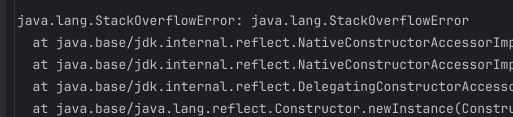
\includegraphics[width=0.8\textwidth]{images/stackOverFlow.jpg}
    \end{figure}

    \subsection{Impacto}

  \section{Pruebas y Resultados}

  \section{Conclusiones}

\end{document}